\documentclass[convert, border=7pt]{standalone}
\usepackage{tikz}
\usepackage{tkz-euclide}

\begin{document}
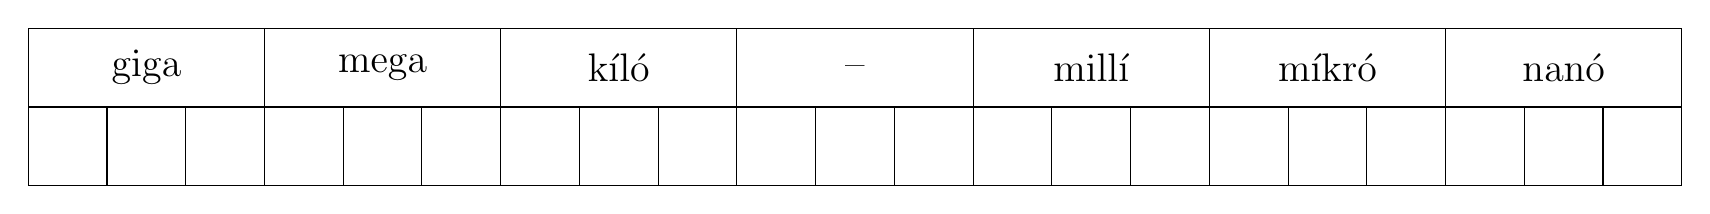
\begin{tikzpicture}

\node (c) at (1.5,1.5) {\Large giga};
\node (c) at (4.5,1.5) {\Large mega};
\node (c) at (7.5,1.5) {\Large kíló};
\node (c) at (10.5,1.5) {\Large --};
\node (c) at (13.5,1.5) {\Large millí};
\node (c) at (16.5,1.5) {\Large míkró};
\node (c) at (19.5,1.5) {\Large nanó};

\foreach \x in {0,1,2}{
\draw (0,\x) -- (21,\x);
};
\foreach \x in {0,3,6,9,12,15,18,21}{
\draw (\x,1) -- (\x,2);
};
\foreach \x in {0,1,2,3,4,5,6,7,8,9,10,11,12,13,14,15,16,17,18,19,20,21}{
\draw (\x,0) -- (\x,1);
};

\end{tikzpicture}
\end{document}
